% SC3010 --- Chapter 4: Access Control (0->100 ground-up)
\chapter{Access Control: ACLs, RBAC, ABAC and Lattices}
\label{ch:access}

\begin{quote}
\emph{``Authentication tells you who they are; access control tells you what they may do.''} --- Every request passes a reference monitor that checks a policy. We build those policies from first principles.
\end{quote}

\noindent\fbox{\parbox{\dimexpr\linewidth-2\fboxsep-2\fboxrule}{%
\textbf{From zero: no prior security model assumed.} We start from a spreadsheet of who may do what, then fold it by columns (ACLs) and rows (capabilities), group by job (RBAC), generalise by attributes (ABAC), and finally order sensitivity in a lattice (Bell--LaPadula/Biba). Pictures first, then definitions, then code.}}
\vspace{0.4em}

\section*{Learning Outcomes}
After this chapter you will be able to:
\begin{enumerate}[label=(L\arabic*)]
    \item define the access matrix and derive ACLs and capability lists as dual views;
    \item model roles, hierarchies, and constraints in RBAC and decide when it fits;
    \item author ABAC policies over subject/object/environment attributes;
    \item draw a security lattice and apply BLP (no read-up, no write-down) and Biba;
    \item choose among ACL/RBAC/ABAC/capabilities for a given system and argue trade-offs.
\end{enumerate}

% ============================================================
\section{The Access Matrix: Columns Are ACLs, Rows Are Capabilities}
\label{sec:matrix}
\paragraph{Intuition.} Write a table: rows $=$ subjects (Alice, Bob), columns $=$ objects (fileA, printer), cells $=$ rights $\{r,w,x\}$. This \emph{access matrix} $M[S,O]$ is the conceptual truth; every real mechanism is a way to store it.

\begin{definition}[Access matrix and its projections]
$M:S\times O\to 2^{R}$ maps each subject--object pair to a set of rights. Column $M[\cdot,O]$ stored with $O$ is an \emph{ACL}; row $M[S,\cdot]$ held by $S$ is a \emph{capability list}. Both encode the same $M$.
\end{definition}

\begin{figure}[h]\centering
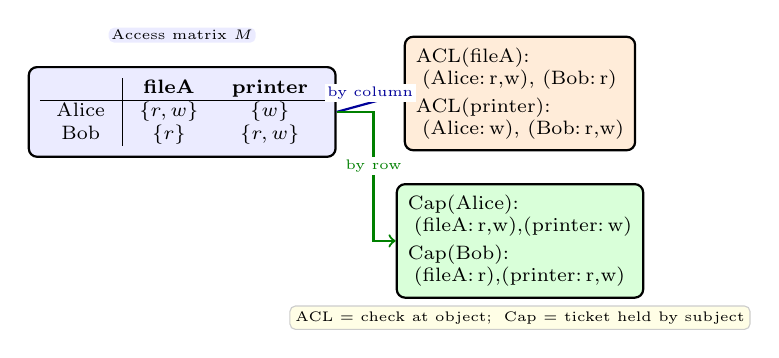
\begin{tikzpicture}[scale=0.78,every node/.style={font=\scriptsize}]
% Matrix
\node[draw,thick,fill=blue!8,rounded corners=3pt,inner sep=4pt] (mat) at (0,1.2) {
\begin{tabular}{c|cc}
 & \textbf{fileA} & \textbf{printer}\\\hline
Alice & $\{r,w\}$ & $\{w\}$\\
Bob   & $\{r\}$   & $\{r,w\}$
\end{tabular}};
\node[font=\tiny,fill=blue!8,rounded corners=2pt,inner sep=1pt] at (0,2.45) {Access matrix $M$};
% ACL view
\node[draw,thick,fill=orange!15,rounded corners=3pt,align=left,inner sep=4pt] (acl) at (5.5,1.5) {ACL(fileA):\\ \;(Alice:\,r,w), (Bob:\,r)\\[2pt] ACL(printer):\\ \;(Alice:\,w), (Bob:\,r,w)};
\draw[->,thick,blue!60!black] (mat.east) -- (acl.west) node[midway,above,font=\tiny,fill=white,inner sep=1pt] {by column};
% Cap view
\node[draw,thick,fill=green!15,rounded corners=3pt,align=left,inner sep=4pt] (cap) at (5.5,-0.9) {Cap(Alice):\\ \;(fileA:\,r,w),(printer:\,w)\\[2pt] Cap(Bob):\\ \;(fileA:\,r),(printer:\,r,w)};
\draw[->,thick,green!50!black] (mat.east) -- ++(0.6,0) |- (cap.west) node[pos=0.25,above,font=\tiny,fill=white,inner sep=1pt] {by row};
\node[font=\tiny,fill=yellow!10,draw=gray!40,rounded corners=2pt,inner sep=2pt] at (5.5,-2.15) {ACL $=$ check at object;\; Cap $=$ ticket held by subject};
\end{tikzpicture}
\caption{One abstract matrix, two storage duals. ACLs live with the object and are checked on access; capabilities live with the subject and are presented like tickets. Colour: blue truth, orange column view, green row view.}
\label{fig:matrix-dual}
\end{figure}

ACLs are natural when objects have owners (Unix \texttt{rwx}, NTFS ACLs) but checking ``what can Alice access?'' scans all ACLs. Capabilities answer that in $O(1)$ but need revocation (how to take a ticket back?)---indirection via a capability table or short expiry. Hybrid systems keep both.

\begin{example}[Unix and Windows ACLs]
Unix ``\texttt{rwx}'' for user/group/other is a compressed ACL with three entries; POSIX ACLs extend to \texttt{setfacl -m u:alice:rw fileA}. Windows NTFS stores per-file DACLs with SIDs and inheritance. Capabilities appear as file descriptors in Unix (if you hold fd~3 you can read) and as object handles in microkernels (seL4, Fuchsia).
\end{example}

\begin{definition}[Reference monitor]
A reference monitor is tamper-proof, always invoked, and small enough to verify (Neumann). It sits on every access path (Fig.~\ref{fig:matrix-dual} arrow) and consults the policy store; bypassing it breaks the model regardless of how clever the policy is.
\end{definition}

\begin{lstlisting}[language=Python,caption={ACL vs.\ capability checks (same matrix, dual lookup).},label={lst:acl-cap}]
M = {("Alice","fileA"):{'r','w'}, ("Alice","printer"):{'w'},
     ("Bob","fileA"):{'r'},       ("Bob","printer"):{'r','w'}}
def acl_check(obj, subj, op):   # object stores its column
    acl = {s: r for (s,o),r in M.items() if o==obj}
    return op in acl.get(subj, set())
def cap_check(subj, obj, op):   # subject holds its row (ticket)
    caps = {o: r for (s,o),r in M.items() if s==subj}
    return op in caps.get(obj, set())
assert acl_check("fileA","Alice",'w') == cap_check("Alice","fileA",'w')
\end{lstlisting}

% ============================================================
\section{RBAC: Roles as Indirection}
\label{sec:rbac}
\paragraph{Intuition.} In a hospital, permissions follow the job, not the person. Alice \emph{has} role Doctor, so she inherits read(chart), write(prescription). When Alice moves to Admin, we move one role assignment, not hundreds of ACL entries.

\begin{definition}[RBAC$_{0}$--RBAC$_{3}$]
Core RBAC$_{0}$: users $U$, roles $R$, permissions $P$, relations $UA\subseteq U\times R$ and $PA\subseteq P\times R$; a session maps a user to a subset of assigned roles. Hierarchy (RBAC$_{1}$) orders $R$ by $\succeq$ (senior inherits junior). Constraints (RBAC$_{2}$) add separation of duty; RBAC$_{3}$ combines both.
\end{definition}

\begin{figure}[h]\centering
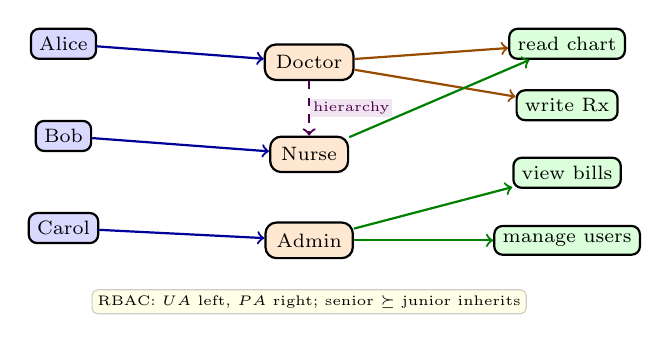
\begin{tikzpicture}[scale=0.78,every node/.style={font=\scriptsize},
  user/.style={draw,thick,fill=blue!15,rounded corners=3pt,inner sep=3pt},
  role/.style={draw,thick,fill=orange!18,rounded corners=4pt,inner sep=4pt},
  perm/.style={draw,thick,fill=green!14,rounded corners=3pt,inner sep=3pt}]
\node[user] (alice) at (0,1.5) {Alice}; \node[user] (bob) at (0,0) {Bob}; \node[user] (carol) at (0,-1.5) {Carol};
\node[role] (doc) at (4,1.2) {Doctor}; \node[role] (nurse) at (4,-0.3) {Nurse}; \node[role] (admin) at (4,-1.7) {Admin};
\node[perm] (p1) at (8.2,1.5) {read chart}; \node[perm] (p2) at (8.2,0.5) {write Rx}; \node[perm] (p3) at (8.2,-0.6) {view bills}; \node[perm] (p4) at (8.2,-1.7) {manage users};
\draw[->,thick,blue!60!black] (alice)--(doc); \draw[->,thick,blue!60!black] (bob)--(nurse); \draw[->,thick,blue!60!black] (carol)--(admin);
\draw[->,thick,orange!60!black] (doc)--(p1); \draw[->,thick,orange!60!black] (doc)--(p2);
\draw[->,thick,green!50!black] (nurse)--(p1); \draw[->,thick,green!50!black] (admin)--(p3); \draw[->,thick,green!50!black] (admin)--(p4);
% hierarchy
\draw[->,thick,violet!60!black,dashed] (doc) -- (nurse) node[midway,right,font=\tiny,fill=violet!10,inner sep=1pt] {hierarchy};
\node[font=\tiny,fill=yellow!10,draw=gray!40,rounded corners=2pt,inner sep=2pt] at (4,-2.7) {RBAC: $UA$ left, $PA$ right; senior $\succeq$ junior inherits};
\end{tikzpicture}
\caption{RBAC indirection. Users assigned to roles ($UA$), roles to permissions ($PA$). Changing a user's job means one $UA$ edit, not many $PA$ edits. Dashed edge shows role hierarchy.}
\label{fig:rbac}
\end{figure}

Separation of duty: \emph{static} (no user in both Purchaser and Approver) prevents fraud even off-session; \emph{dynamic} (same session may not activate both) is more flexible. RBAC shines when roles are stable and auditable, but explodes when permissions need fine attributes (``doctors may read charts of patients in their ward between 9--5'')---that is ABAC territory.

\begin{example}[Role explosion]
A university with departments $\times$ courses $\times$ $\{student,TA,instructor\}$ na\"ively needs $D\cdot C\cdot 3$ roles. With hierarchy (Instructor $\succeq$ TA $\succeq$ Student per course) plus parameterised roles (\texttt{Instructor(CS101)}), count drops to $O(D+C)$. Without this, RBAC degenerates into per-user ACLs.
\end{example}

% ============================================================
\section{ABAC: Policies over Attributes}
\label{sec:abac}
\paragraph{Intuition.} Instead of naming roles, write a rule on \emph{attributes}: subject attrs (dept, clearance), object attrs (owner, classification), environment attrs (time, location), and an action. A Policy Decision Point evaluates: $\text{permit iff } \text{policy}(sub, obj, env, act)=\text{true}$.

\begin{definition}[ABAC policy]
Let $A_s,A_o,A_e$ be attribute sets. A policy is a predicate $P: A_s\times A_o\times A_e\times Act\to\{\text{permit},\text{deny}\}$. The reference monitor calls $P$ on every access; combining algorithms (deny-overrides, permit-overrides) resolve multiple policies.
\end{definition}

\begin{lstlisting}[language=Python,caption={ABAC policy: attribute rule with combining.},label={lst:abac}]
def policy(sub, obj, env, act) -> bool:
    # Rule: doctors in same ward, during shift, may read charts
    if sub["role"]=="doctor" and obj["type"]=="chart" and act=="read":
        if sub["ward"]==obj["ward"] and 9 <= env["hour"] < 17:
            return True
    # Rule: owner may always read own record
    if sub["id"]==obj["owner"] and act=="read":
        return True
    return False  # default deny (closed policy)

# PDP: deny-overrides if any deny policy triggers; here single policy
def pdp(sub,obj,env,act): return "permit" if policy(sub,obj,env,act) else "deny"
\end{lstlisting}
ABAC generalises ACL and RBAC: an ACL is ``attr $=$ identity'', a role is one subject attribute. Price: policy review is harder (attribute sprawl, conflicting rules, time-of-check--time-of-use). XACML/OPA/Rego are industry policy languages; minimal, testable, version-controlled policies are essential.

\begin{remark}[Combining and default deny]
With multiple rules, \emph{deny-overrides} (any deny $\Rightarrow$ deny) is safest for closed policies; \emph{permit-overrides} suits open collaborations. NIST 800-162 recommends a default deny and explicit permit rules, plus a \emph{break-glass} override (audited emergency permit) that temporarily bypasses deny.
\end{remark}

% ============================================================
\section{Lattice Model: Classifying Information Flow}
\label{sec:lattice}
\paragraph{Intuition.} Some data is more sensitive than other data: {\small Public $\sqsubset$ Confidential $\sqsubset$ Secret $\sqsubset$ Top Secret}, and compartments add dimensions (e.g.\ Crypto, Nuclear). Sensitivity forms a \emph{lattice}: any two labels have a least upper bound (join $\sqcup$) and greatest lower bound (meet $\sqcap$). Information may only flow \emph{up} the lattice.

\begin{definition}[Security lattice]
A lattice $(L,\sqsubseteq)$ is a partial order where every pair $a,b$ has $\sup\{a,b\}=a\sqcup b$ and $\inf\{a,b\}=a\sqcap b$. Labels are $\ell=(level, compartments)$ with $\ell_1\sqsubseteq\ell_2$ iff $level_1\le level_2$ and $compartments_1\subseteq compartments_2$.
\end{definition}

Two classic uses read the lattice in opposite directions:
\begin{itemize}[leftmargin=*, itemsep=0.25em]
    \item \textbf{Bell--LaPadula (confidentiality):} no read-up, no write-down. Subject $S$ with clearance $\lambda(S)$ may read object $O$ only if $\lambda(O)\sqsubseteq\lambda(S)$ (Simple Security) and write only if $\lambda(S)\sqsubseteq\lambda(O)$ (Star Property). Prevents leaking Secret into Public.
    \item \textbf{Biba (integrity):} dual---no read-down, no write-up. Low-integrity data must not contaminate high-integrity decisions.
\end{itemize}

\begin{figure}[h]\centering
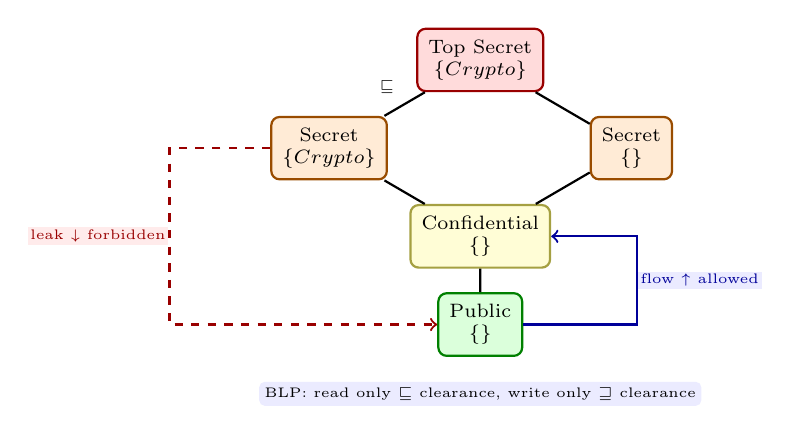
\begin{tikzpicture}[scale=0.80,every node/.style={font=\scriptsize},
  lvl/.style={draw,thick,rounded corners=3pt,align=center,inner sep=4pt}]
% Lattice Hasse
\node[lvl,fill=red!14,draw=red!60!black] (ts) at (4,3.2) {Top Secret\\ $\{\text{Crypto}\}$};
\node[lvl,fill=orange!16,draw=orange!60!black] (s1) at (1.6,1.8) {Secret\\ $\{\text{Crypto}\}$};
\node[lvl,fill=orange!16,draw=orange!60!black] (s2) at (6.4,1.8) {Secret\\ $\{\}$};
\node[lvl,fill=yellow!16,draw=yellow!60!black] (c) at (4,0.4) {Confidential\\ $\{\}$};
\node[lvl,fill=green!14,draw=green!50!black] (pub) at (4,-1.0) {Public\\ $\{\}$};
\draw[thick] (ts)--(s1) node[midway,above left,font=\tiny] {$\sqsubseteq$};
\draw[thick] (ts)--(s2);
\draw[thick] (s1)--(c); \draw[thick] (s2)--(c); \draw[thick] (c)--(pub);
% flow arrows
\draw[->,thick,blue!60!black] (pub.east) -- ++(1.8,0) |- (c.east) node[pos=0.25,right,font=\tiny,fill=blue!8,inner sep=1pt] {flow $\uparrow$ allowed};
\draw[->,thick,red!60!black,dashed] (s1.west) -- ++(-1.6,0) |- (pub.west) node[pos=0.25,left,font=\tiny,fill=red!8,inner sep=1pt] {leak $\downarrow$ forbidden};
% legend
\node[font=\tiny,fill=blue!8,rounded corners=2pt,inner sep=2pt] at (4,-2.1) {BLP: read only $\sqsubseteq$ clearance, write only $\sqsupseteq$ clearance};
\end{tikzpicture}
\caption{Hasse diagram of a security lattice (levels $\times$ compartments). Information flows upward; BLP forbids downward flow (red dashed). Join of the two Secret nodes is the TS node. The diagram is a ``ravioli'' stacking of levels with compartment sets.}
\label{fig:lattice}
\end{figure}

\begin{theorem}[BLP enforces no downward leak]
If all reads satisfy $\lambda(O)\sqsubseteq\lambda(S)$ and writes satisfy $\lambda(S)\sqsubseteq\lambda(O)$, and labels are monotone (tranquillity: labels do not change to leak), then no sequence of operations copies data from higher to strictly lower label.
\end{theorem}
Real systems relax strict BLP with \emph{trusted subjects} (downgraders) that are verified to sanitise, and handle covert channels (timing, resource exhaustion) outside the lattice. Multilevel databases and SELinux MLS/MCS implement lattice ideas at OS granularity.

\begin{example}[Covert channel outside the lattice]
BLP stops explicit read/write, but a Top Secret process can signal one bit to a Public process by modulating CPU load (high $=$ 1, low $=$ 0) if they share a scheduler. The data \emph{flow} is not via a labelled object, so the lattice does not see it. Mitigation: partition resources, add noise, or bound channel capacity (Lampson, 1973).
\end{example}

% ============================================================
\section{Exercises}
\label{sec:access-exercises}
\begin{enumerate}[label=E4.\arabic*, leftmargin=*, itemsep=0.6em]
    \item \textbf{ACL vs.\ capability audit.} Given $M$ with 1000 subjects and $10^5$ files averaging 10 entries per ACL, compute cost of ``list all files Alice can write'' via ACL scan vs.\ capability cache. Propose a hybrid that keeps ACLs authoritative but caches per-subject lists, and explain revocation.
    \item \textbf{RBAC separation of duty.} Design RBAC for a bank: roles Teller, Auditor, Manager with permissions post/withdraw/audit/approve-loan. State static and dynamic SoD constraints that prevent (a) self-audit and (b) single-person loan fraud. Show a violating $UA$ assignment.
    \item \textbf{ABAC policy authoring.} Write an ABAC rule: ``Nurses may write vitals for patients in their ward during their shift, and patients may read their own chart anytime.'' Identify subject/object/environment attributes, give allow/deny test cases, and show a conflict where both an allow and deny rule fire; apply deny-overrides.
    \item \textbf{Lattice join/meet.} For $L=\{Public, Confidential, Secret\}\times\mathcal{P}(\{Med,Fin\})$ ordered by level and $\subseteq$ on compartments, compute $(Secret,\{Med\})\sqcup(Confidential,\{Fin\})$ and $\sqcap$, and list all labels $\sqsubseteq(Secret,\{Med,Fin\})$.
    \item \textbf{BLP vs.\ Biba trade-off.} A system must enforce both confidentiality (BLP) and integrity (Biba) on the same lattice. Show that the combined rules forbid any read or write between distinct levels, and propose how real systems (e.g.\ SELinux) handle this by separating confidentiality and integrity lattices or using trusted subjects.
\end{enumerate}

% ============================================================
\section*{Chapter Notes}
Lampson (1971) introduced the access matrix and its ACL/capability duality; Saltzer--Schroeder (1975) framed the reference monitor. RBAC was systematised by Ferraiolo--Kuhn (1992) and standardised as ANSI INCITS~359 (RBAC$_{0}$--$_{3}$). ABAC generalises both and underpins NIST 800-162 and OPA/Rego. Denning (1976) formalised lattices for information flow; Bell--LaPadula (1973, MITRE) and Biba (1977) are the confidentiality/integrity duals. For SELinux MLS see Mayer--MacMillan--Caplan; for capabilities see Levy (1984) and modern Capsicum/CHERI.
% End of Chapter 4
% SC3010-Ch04 access control — lattice as ravioli stacking of levels $\times$ compartments.
